This section describes how the speedup techniques were explored and describes how we came up with the proposed EMS-GT2 algorithm. This also describes the process in evaluating the speedup techniques as well as other algorithms that solve the $(l, d)$-planted motif problem.

% Each algorithm was evaluated using the $(9, 2)$, $(11, 3)$, $(13, 4)$, $(15, 5)$ and $(17, 6)$ challenge instances. 

\begin{figure}[h]
	\centering
	\label{fig:methodology}
	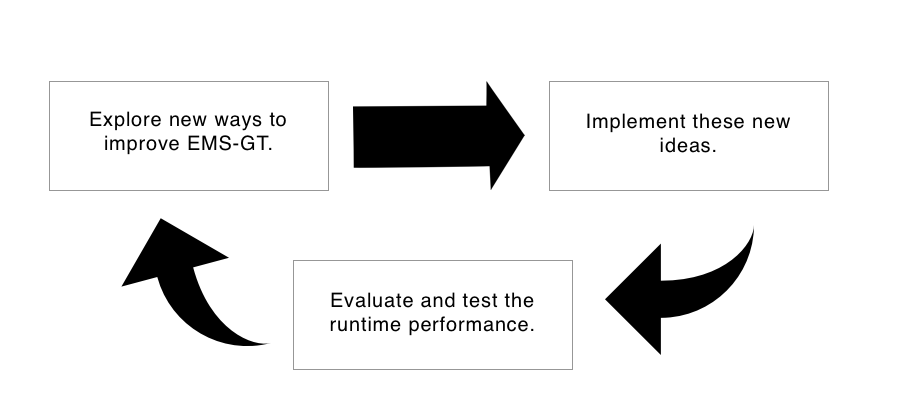
\includegraphics[width=5.5in]{contents/00_images/methodology}
	\caption{Speedup Technique Development Cycle.}
\end{figure} 

The study aims to improve the algorithm by pre-computation of values and exploring other usage of the block-processing technique. The speedup techniques were developed following the cycle shown in Figure \ref{fig:methodology}.

\section{Improving the EMS-GT algorithm}
%  C++ implementation
Originally, EMS-GT was implemented using Java, but for the purpose of eliminating unnecessary variables that may affect the evaluation of the algorithms, it was converted to C++. This is the same language used in the development of the PMS8 and qPMS9 algorithms.

% block flags
A previous study \cite{sia2015} improved the neighborhood generation of an $l$-mer by the use of block bits settings in the neighborhood array instead of one bit at a time. The Generation phase quickly filters the candidate motifs array as it processes the first $n'$ sequences, leaving numerous empty blocks of $l$-mers in the candidate motifs array. It was observed that at some point in the Generation phase, some of the block settings are not necessary anymore since that block is already empty in the candidate motifs array. We improved the algorithm by maintaining boolean flags for those empty blocks and then we skip all block bit settings for those blocks. Additionally, the block-processing procedure was found useful in testing of candidate motifs. The Test phase checks if a candidate motif $c$ is in the remaining $n - n'$ sequences by comparing if there is at least one $l$-mer in each sequence that is within $d$-distance from $c$. If a candidate motif $x$ is eliminated for failing to have a $d$-neighbor in some input sequence $S_i$, that it is possible to reduce the testing for another candidate motif $y$ on the same sequence $S_i$, if $y$ is within the same $k$-block as $x$.

% pre computation
Lastly, hamming distance computation was also improved using a pre-computed lookup values. Given an XOR result, instead of counting nonzero pairs of bits, we use the lookup table to get the number of mismatches. 

% n' values then parameter fine tuning

\section{Parameter Fine Tuning}
The EMS-GT algorithm defines an integer value $n'$ ($1 \leq n' \leq n$) that divides the dataset into two smaller set of sequences. The first $n'$ sequences are used in the Generate phase while the remaining sequences are assigned to the Test phase. Previous experimentations \cite{sia2015} showed that it is efficient for the algorithm to use $n' = 10$. Technically, the $n'$ parameter is related to the candidate motifs array $\mathcal{C}$ size that will be evaluated in the remaining $n - n'$ sequences.

In this study, we re-evaluated the ideal value for $n'$, since two of the speedup techniques introduced here requires sufficiently large candidate motifs array for them to take effect. We run an experimentation that records the average runtime of the algorithm with the speedup techniques over 5 tests and having different values for $n'$. The values for $n'$ ranges from 5 to 10 in this experiment.

Table 3.\ref{tbl:nprime-speedup} shows the ideal $n'$ values for each ($l$, $d$)-challenge instances mentioned. For $(l, d)$ instances where $l \leq 11$, the ideal value for $n'$ is still 10. This is true due to the efficiency of the Generate phase in small instances of the problem. For (13, 4), (15, 5) and (17, 6) problem instances, different $n'$ values were used in the evaluation which are 9, 8, and 7 respectively.

\begin{table}[h] %Empty Blocks
	\renewcommand{\arraystretch}{1.3}
	\label{tbl:nprime-speedup}
	\centering
	\begin{tabular}{|c|c|c|c|c|c|}
		\hline 
		\bfseries\boldmath $Sequence$ & 
		\bfseries\boldmath $(9,2)$ & 
		\bfseries\boldmath $(11,3)$ & 
		\bfseries\boldmath $(13,4)$ & 
		\bfseries\boldmath $(15,5)$ & 
		\bfseries\boldmath $(17,6)$ \\
		\hline
			5	& 	0.07 s			& 	0.42 s 			&	2.37 s			&	17.86 s				&	148.62 s\\
			6	& 	0.06 s			& 	0.29 s			& 	1.54 s			&	12.64 s				&	116.01 s\\
			7	& 	0.05 s			& 	0.21 s			& 	1.01 s			&	10.70 s				&	\textbf{111.94 s}\\
			8	& 	0.05 s			&	0.18 s			& 	0.84 s			&	\textbf{10.38 s}	&	119.82 s\\
			9	& 	0.03 s 			& 	0.14 s			& 	\textbf{0.75 s}	&	11.01 s				&	132.10 s\\
			10	& 	\textbf{0.03 s} &	\textbf{0.13 s}	& 	0.76 s			&	11.90 s				&	146.10 s\\
		\hline\end{tabular}
	\caption{Runtime evaluation of the algorithm with speedup over different $n'$ values.}
\end{table}

Additionally, the block flags speedup technique also defines another parameter $n''$ where $1 \leq n'' \leq n'$. This parameter represents the sequence number where the algorithm will start using the block flags. We also run an experimentation to assess the best value for the parameter $n''$. Table 3.\ref{tbl:nprime-prime-start-value} shows the runtime performance of EMS-GT with the block flags speedup technique using different $n''$ values. The experiments showed that the ideal value for $n''$ in instances (9, 2), (11, 3), (13, 4), (15, 5) and (17, 6) are 8, 10, 7, 7 and 7 respectively.

% nprime_prime-speedup
\begin{table}[h] %Empty Blocks
	\renewcommand{\arraystretch}{1.3}
	\label{tbl:nprime-prime-start-value}
	\centering
	\begin{tabular}{|c|c|c|c|c|c|}
		\hline 
		\bfseries\boldmath $Sequence$ & 
		\bfseries\boldmath $(9,2)$ & 
		\bfseries\boldmath $(11,3)$ & 
		\bfseries\boldmath $(13,4)$ & 
		\bfseries\boldmath $(15,5)$ & 
		\bfseries\boldmath $(17,6)$ \\
		\hline
			2	& 0.039	s & 0.138 s & 1.006	s & 14.255 s &	149.369 s\\
			3	& 0.034	s & 0.136 s & 1.067	s & 13.888 s &	143.152 s\\
			4	& 0.038	s & 0.129 s & 0.947	s & 13.274 s &	137.835 s\\
			5	& 0.036	s & 0.121 s & 0.969	s & 12.972 s &	134.219 s\\
			6	& 0.037	s & 0.119 s & 0.887	s & 12.776 s &	132.306 s\\
			7	& 0.037	s & 0.120 s & \textbf{0.878	s} & \textbf{12.422 s} &	\textbf{132.207 s}\\
			8	& \textbf{0.032	s} & 0.115 s & 0.928	s & 12.451 s &	135.140 s\\
			9	& 0.036	s & 0.106 s	& 0.891	s & 12.775 s &	138.997 s\\
			10	& 0.035	s & \textbf{0.104 s}	& 0.914 s &	13.054 s &	143.720 s\\
		\hline\end{tabular}
	\caption{Runtime evaluation of the algorithm with the block boolean flags strategy and pre-computed hamming distance over different $n''$ values.}
\end{table}

\section{Evaluation}
We evaluated each of the speedup techniques introduced in this study. We combined these speedup techniques and determined which combination yields the fastest runtime performance, which will be incorporated in the proposed EMS-GT2 algorithm. Specifically, these different combinations are the following: (1) EMS-GT with block boolean flags, (2) EMS-GT with block boolean flags and improved Hamming distance computation, (3) EMS-GT with fast candidate motif elimination, (4) EMS-GT with fast candidate motif elimination and improved Hamming distance computation and (5) EMS-GT with block boolean flags, fast candidate motif elimination and improved Hamming distance computation. We also evaluated EMS-GT2 with its predecessor EMS-GT and with the qPMS9 algorithm.

\section{Datasets}

The algorithm EMS-GT2 was evaluated using both synthetic datasets and real datasets.

\subsection{Synthetic Datasets}
Algorithms that solve PMS \cite{pevzner2000combinatorial, pms2014, pms2015} use a dataset containing $20$ string sequences where each nucleotide is in $\Sigma = \{a, c, g, t\}$. Each string sequence is $600$ base pairs (bp) long and each nucleotide is randomly generated with equal chance of being selected. A motif is then generated and for each string sequence in the dataset, a $d$-neighbor is planted at a random position. In this study, a generator was run to produce a dataset of PMS problem instances with this configuration, and this dataset was then used to evaluate the algorithms. Furthermore, a converter program was used to translate the dataset into FASTA format in order to execute qPMS9.


\subsection{Real Datasets}
% The EMS-GT algorithm was previously evaluated using real data sets. In the EMS-GT2 algorithm, we re-evaluated the runtime performance of the algorithm using the same real data sets. 

The EMS-GT2 algorithm was also evaluated using real datasets that were previously used in the earlier implementation of EMS-GT. The real datasets are the sets of promoter sequences of yeast (\textit{Saccharomyces cervisiae}) \cite{zhu1999scpd} and sets of orthologous sequences of different gene families of eukaryotes. The study \cite{nabos2015dissertation} used these real datasets.



